\begin{appendix}
\chapter{Anhang}
\label{chap:anhang}

\section{Flächenflugzeug}
Der in Gleichung \ref{eq:geschw_flaechenflugzeug} aufgeführte Zusammenhang entsteht aus dem Verhältnis der Fluggeschwindigkeiten bei konstanten Auftriebsbeiwert. Aus der Definition des Auftriebsbeiwertes
\begin{equation}
	c_{A} = \frac{A}{\rho/2\cdot V^2\cdot S}
\end{equation}
entsteht durch Umformen die Beziehung für die Geschwindigkeit
\begin{equation}
	V = \sqrt{\frac{2\cdot A}{\rho\cdot S \cdot c_{A}}} \eqend{.}
\end{equation}
Im Horizontalflug (\ensuremath{\gamma = 0}) kompensiert der Auftrieb lediglich die Gewichtskraft (Vgl. Gleichung \ref{eq:auftriebsgleichung_vereinfacht})
\begin{equation}
	A = G \eqend{.}
\end{equation}
Für jegliche Art von Steigflug (\ensuremath{\gamma \neq 0}) ist dies nicht mehr der Fall. Unter der Voraussetzung einer gleichen Gewichtskraft \ensuremath{m\cdot g}, gleicher Flügelfläche \ensuremath{S} und einem konstanten Auftriebsbeiwerts \ensuremath{c_{A}} ergibt sich für das Verhältnis der Geschwindigkeiten \ensuremath{V/V^\star}
\begin{equation}
	\frac{V}{V^\star} = \frac{\sqrt{\frac{2\cdot m \cdot g\cdot \cos\gamma}{\rho\cdot S \cdot c_{A}}}}{\sqrt{\frac{2\cdot m\cdot g}{\rho^\star \cdot S \cdot c_{A}}}} = \sqrt{\cos\gamma\cdot\frac{\rho^\star}{\rho}} \eqend{.}
\end{equation}

\section{Steiggeschwindigkeit}
\begin{center}
\begin{figure}[H]
\begin{struktogramm}(163,160)
\while[5]{Für alle Bahngeschwindigkeiten}
	\assign[2]{Berechne Gesamtmasse}
	\assign[2]{Flugzeit für Höhenschritt berechnen}			
	\while[5]{Solange Abbruchkriterium nicht erreicht}
		\assign{Aerodynamik berechnen}
	\whileend
	\assign[2]{Schub berechnen}
	\assign[2]{Schub auf Propeller verteilen}
	\ifthenelse[10]{1}{4}{Schub zu gro\ss{}?}{ja}{nein}
		\assign[2]{Ergebnis verwerfen (NaN)}
		\change
		\assign[2]{Drehzahl und Drehmoment aus Propellerkennfeld interpolieren}
		\assign[2]{Motorzustand berechnen}
		\assign[2]{Zustand der Motorregler berechnen}
		\assign[2]{Zustand der Batterie neu berechnen}
		\assign[2]{Gesamtwirkungsgrad berechnen}
	\ifend
	\ifthenelse[10]{1}{1}{Werden Grenzen überschritten?}{ja}{nein}
		\assign[2]{Ergebnis verwerfen (NaN)}
		\change
		\assign[2]{Ergebnis beibehalten}
	\ifend
	\assign[2]{Speichern der aufgebrachten Energiemenge}
\whileend
\ifthenelse[10]{5}{1}{Sind die Werte NaN?}{nein}{ja}
	\while[5]{Solange Abbruchkriterium nicht erreicht}		
		\assign[2]{Finde den Index mit der geringsten verbrauchten Energiemenge}
		\ifthenelse[10]{1}{3}{Werte innerhalb Leistungsgrenzen?}{ja}{nein}
			\assign[2]{Verlasse Schleife}
			\change
			\assign[2]{Suche nächst kleinere Energiemenge}
		\ifend
	\whileend
	\assign[2]{Übergabe aller Leistungsparameter mit diesem Index}
		\change
	\assign[2]{Verwerfe alle Ergebnisse}
\ifend
\end{struktogramm}
\caption{Programmstruktur zur Ermittlung der optimalen Steiggeschwindigkeit}
\label{abb:steiggeschw}
\end{figure}
\end{center}

\section{Batteriemasse}
\begin{figure}[H]
\centering
	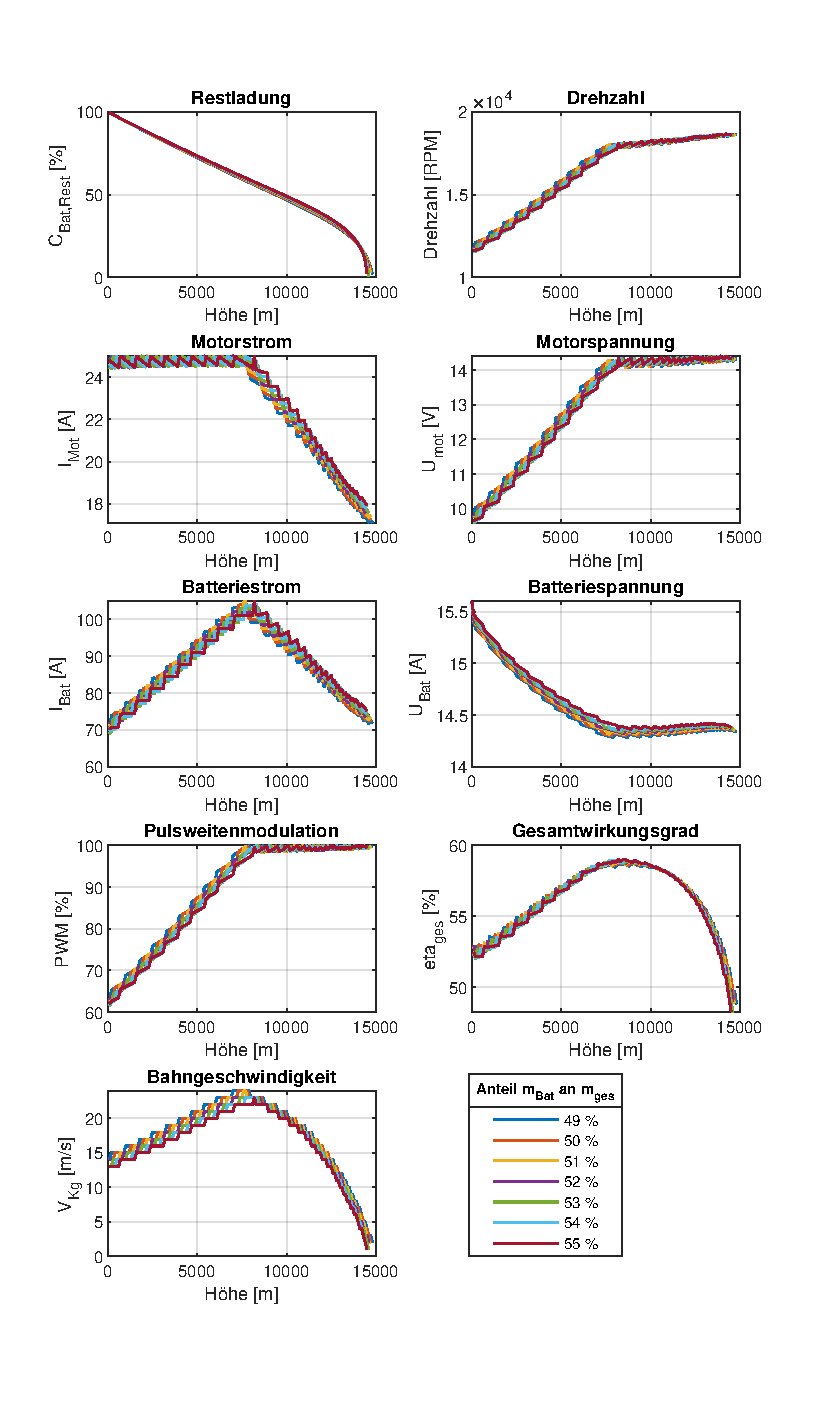
\includegraphics[scale=0.85]{Diagramme/Batteriemasse_genauer.pdf}
	\caption{genauere Untersuchung der Batteriemassenabhängigkeit (\ensuremath{m_{Mot}=\SI{106}{g}}, \ensuremath{K_V=\SI{1390}{RPM/V}}, \ensuremath{n_{Prop}=4}, \ensuremath{Propeller=\SI{10x3}{}}, \ensuremath{n_{Bat,cell}=4}, \ensuremath{u_{Wg}=\SI{10}{m/s}})}
	\label{abb:batteriemasse_genauer}
\end{figure}





\end{appendix}
